\documentclass[ignorenonframetext,red]{beamer}

\usepackage{ucs}
\usepackage{mathpartir}
\usepackage{amsfonts,amsmath}
\usepackage{stmaryrd}
\usepackage[utf8x]{inputenc}
\usepackage[protrusion=true,expansion=true]{microtype}
\usepackage{setspace}
\usepackage{graphicx}
\usepackage{natbib}
\usepackage{listings}

\usepackage{../../macros}

\date{\\[1em] May 2011 \\[1em]
\scriptsize CEA LIST}

\title{A logical framework for incremental type-checking}

\author[Matthias Puech \& Yann Régis-Gianas] {
  Matthias Puech\inst{1,2} \and Yann Régis-Gianas\inst{2}
}

\institute {
  \inst 1 {Dept. of Computer Science, University of Bologna} \and
  \inst 2 {University Paris 7, CNRS, and INRIA, PPS, team ${\pi}r^2$}
}

\setbeamertemplate{footline}[frame number]
\setbeamertemplate{navigation symbols}{}
\setbeamertemplate{itemize item}[circle]

\usefonttheme{serif}

\AtBeginSection[]
{\begin{frame}<beamer>{Menu}
    \tableofcontents[currentsection]
  \end{frame}
}
\lstset{
  language=[Objective]Caml,
  basicstyle=\sf,
  columns=flexible,
  literate={->}{{$\to$ }}1 {*}{$\times$ }1 {>=}{{$\geq$}}1
  {<>}{{$\neq$}}1 {'a}{{$\alpha$}}1 {'b}{{$\beta$}}1 {'c}{{$\gamma$}}1
}

\begin{document}

\frame\titlepage


\begin{frame}{A paradoxical situation}  
  \begin{block}{Observation}
    We have powerful tools to mechanize the metatheory of (proof) languages
  \end{block}
  \pause
  \begin{block}{\ldots\ And yet,}
    Workflow of programming and formal mathematics is still largely inspired by legacy
    software development (\textsf{emacs}, \textsf{make}, \textsf{svn},
    \textsf{diff}s\ldots)
  \end{block}
  \vspace{0.6em}
  \pause
  \begin{center}
    {\large \it Isn't it time to make these tools metatheory-aware?}
  \end{center}
\end{frame}

\begin{frame}{Incrementality in programming {\it \&} proof languages}
  
  {\Huge Q {\Large :}} \parbox{0.8\textwidth}{Do you spend more time
    \emph{writing} code or \emph{editing} code?} \\[2em]

Today, we use:
  \begin{itemize}
  \item separate compilation
  \item dependency management
  \item version control on the scripts
  \item interactive toplevel with rollback (\textsf{Coq})
  \end{itemize}
\end{frame}

\begin{frame}{Incrementality in programming {\it \&} proof languages}
  \vspace{0.5em}
  \begin{center}
    \only<1>{\includegraphics[width=0.85\textwidth]{images/coqide00.png}}%
    \only<2>{\includegraphics[width=0.85\textwidth]{images/coqide0.png}}%
    \only<3>{\includegraphics[width=0.85\textwidth]{images/coqide.png}}%
    \only<4>{\includegraphics[width=0.85\textwidth]{images/coqide2.png}}%
    \only<5>{\includegraphics[width=0.85\textwidth]{images/coqide4.png}}%
    \only<6>{\includegraphics[width=0.85\textwidth]{images/coqide5.png}}%
    \only<7>{\includegraphics[width=0.85\textwidth]{images/coqide6.png}}%
    \only<8>{\includegraphics[width=0.85\textwidth]{images/coqide7.png}}%
  \end{center}
\end{frame}

\begin{frame}{In an ideal world\ldots}
  \begin{itemize}
  \item Edition should be possible anywhere
  \item The impact of changes visible “in real time”
  \item No need for separate compilation, dependency management
  \end{itemize}
  \pause
  \vspace{2em}
  \begin{center}
    {\large \it Types are good witnesses of this impact}
  \end{center}
  \vspace{1em}
  \pause
  \begin{block}{Applications}
    \small
    \begin{itemize}
    \item non-(linear$|$batch) user interaction
    \item typed version control systems
    \item type-directed programming
    \item tactic languages
    \end{itemize}
  \end{block}
\end{frame}

\begin{frame}{In this talk, we focus on\ldots}
  \ldots\ building a procedure to type-check \emph{local changes}

  \begin{itemize}
  \item What data structure for storing type derivations?
  \item What language for expressing changes?
  \item How to implement basic operations?
  \end{itemize}
\end{frame}

\begin{frame}{Menu}
  \tableofcontents
\end{frame}

\section{The big picture}

\begin{frame}{The big picture}
  \begin{center}
    \only<1-2>{\fbox{\parbox{20em}{\only<2>\alert{version
            management}\\[1em]%
          \fbox{\parbox{18em}{script files\\[1em]%
              \fbox{\parbox{17em}{parsing\\[1em]%
                  \fbox{\parbox{14em}{type-checking\\} }}}}}}}}%
    \only<3>{\fbox{\parbox{20em}{script files\\[1em]%
          \fbox{\parbox{18em}{\alert{version management}\\[1em]%
              \fbox{\parbox{17em}{parsing\\[1em]%
                  \fbox{\parbox{14em}{type-checking\\} }}}}}}}}%
    \only<4-6>{\fbox{\parbox{20em}{
          \begin{overlayarea}{20em}{2em}
            \alt<-5>{script files}{user interaction}
          \end{overlayarea}%
          \fbox{\parbox{18em}{parsing\\[1em]%
              \fbox{\parbox{17em}{\alert{version management}\\[1em]%
                  \uncover<4-6>{\fbox{\parbox{14.5em}{type-checking\\}}}}}}}}}}%
    \only<7->{\fbox{\parbox{20em}{
          \begin{overlayarea}{20em}{2em}
            user interaction
          \end{overlayarea}%
          \fbox{\parbox{18em}{parsing\\[1em]%
              \fbox{\parbox{17em}{\only<8->{incremental }type-checking\\[1em]%
                  \fbox{\parbox{14.5em}{\alert{version management}\\}}}}}}}}}%
  \end{center}
  \begin{itemize}
  \item<4-> AST representation
  \item<7-> Typing annotations
  \end{itemize}
\end{frame}

\subsection{Incremental type-checking}

\begin{frame}[fragile]{\gray{A logical framework for incremental}
    type-checking}
  Yes, we're speaking about (any) typed language.
  \begin{block}{A type-checker}
    \begin{lstlisting}
      val check : env -> term -> types -> bool
    \end{lstlisting}
    \begin{itemize}
    \item builds and checks the derivation (on the stack)
    \item conscientiously discards it
    \end{itemize}
  \end{block}
  \pause
  \def\envbarb{A\to B, B\to C, A\vdash}
  
  \begin{overlayarea}{\textwidth}{7em}
    \alt<-2>{
      \[ \tiny
      \def\impi{{\tiny$\to_i$}}
      \def\impe{{\tiny$\to_e$}}
      \def\ax{{\tiny$Ax$}}
      \infer*[left=\impi]{
        \infer*[left=\impi]{
          \infer*[left=\impi]{
            \infer*[left=\impe]{
              \infer*[right=\ax,leftskip=5em]{ }{\envbarb B\to C}\\
              \infer*[right=\impe,rightskip=5em]{
                \infer*[right=\ax]{ }{\envbarb A\to B}\\
                \infer*[right=\ax]{ }{\envbarb A}
              }{\envbarb B}
            }{\envbarb C}
          }{A\to B, B\to C\vdash A\to C}
        }{A\to B\vdash (B\to C)\to A\to C}
      }{\vdash (A\to B)\to(B\to C)\to A\to C}
      \]
    }{
      \begin{center}
        \vspace{3em}
        \large \textsf{\textbf{true}}
      \end{center}
    }
  \end{overlayarea}
  \pause  
\end{frame}

\begin{frame}{\gray{A logical framework for} incremental
    \gray{type-checking}}
  \begin{onlyenv}<-3>
    \begin{description}
    \item[Goal] Type-check a large derivation taking advantage of the
      knowledge from type-checking previous versions
    \item[Idea] Remember all derivations!
    \end{description}
    \pause \inXLF
    \begin{block}{More precisely}
      Given a well-typed $\mr : repository$ and a $\delta : delta$
      and $$\mathsf{apply} : repository \to delta \to term\ ,$$an
      incremental type-checker $$\mathsf{tc} : repository \to delta
      \to \alt<-2>{bool}{repository\ option} $$ decides if
      $\delta(\mr)$ is
      well-typed in $O(|\delta|)$. \\
      {\hfill\scriptsize (and not $O(|\delta(\mr)|)$)}
    \end{block}
  \end{onlyenv}
  \begin{onlyenv}<4->
    from \\
    {\centering\includegraphics[width=0.5\textwidth]{images/tc-classic.png}\\}
    to \\
    {\centering\includegraphics[width=0.5\textwidth]{images/tc-delta1.png}\\}
  \end{onlyenv}
\end{frame}

\subsection{Why not memoization?}

\begin{frame}[fragile]{Memoization maybe?}
  \begin{onlyenv}<1>
    \vspace{4em}
\begin{lstlisting}
let rec check env t a = 
  match t with
  | ... -> ... false
  | ... -> ... true

and infer env t =
  match t with 
  | ... -> ... None
  | ... -> ... Some a
\end{lstlisting}
  \end{onlyenv}
  \begin{onlyenv}<2>
    \vspace{3em}
\begin{lstlisting}
let table = ref ([] : environ * term * types) in
let rec check env t a = 
  if List.mem (env,t,a) !table then true else
    match t with
    | ... -> ... false
    | ... -> ... table := (env,t,a)::!table; true
and infer env t =
  try List.assoc (env,t) !table with Not_found ->
    match t with 
    | ... -> ... None
    | ... -> ... table := (env,t,a)::!table; Some a
\end{lstlisting}
  \end{onlyenv}
  \pause\pause
  \begin{block}{Syntactically}
    \begin{enumerate}
    \item[\itplus] lightweight, efficient implementation
      \pause
    \item[\itplus] $repository = \mathsf{table}$, $delta =
      \mathsf{t}$
      \pause
    \item [\itminus] syntactic comparison (no quotient on judgements) \\
    {\footnotesize What if I want \emph{e.g.} weakening or
      permutation to be taken into account?}
    \end{enumerate}
  \end{block}
  \pause
  \vspace{-1em}
  \begin{block}{Semantically}
    \begin{enumerate}
    \item[\itminus] external to the type system (meta-cut) \\
      {\footnotesize What does it mean logically?
        \begin{mathpar}
          \tiny
          \infer {J\in \Gamma} {\Gamma\vdash \jwf J\To \Gamma} \and
          \infer {\Gamma_1\vdash \jwf{J_1} \To \Gamma_2\\\ldots\\
            \Gamma_{n-1}[J_{n-1}]\vdash \jwf{J_n}\To \Gamma_n}
          {\Gamma_1\vdash \jwf J\To \Gamma_n[J_n][J]}
        \end{mathpar}
      }
      \pause
    \item[\itminus] imperative (introduces a dissymmetry)
    \end{enumerate}
  \end{block}
  \pause
  {\footnotesize Mixes two goals:} {\large \it derivation synthesis}
  {\footnotesize \&} {\large \it object reuse}
\end{frame}

\section{Our approach}

\subsection{Two-passes type-checking}

\begin{frame}{Two-passes type-checking}

  {\centering\includegraphics[width=0.7\textwidth]{images/tc-delta2.png}\\}
  focus on \textsf{tc}
\end{frame}

\subsection{The data-oriented way}

\begin{frame}{A popular storage model for repositories}
  \begin{onlyenv}<1-7>
    \begin{center}
      \only<+>{\includegraphics[width=0.85\textwidth]{images/git1.pdf}}%
      \only<+>{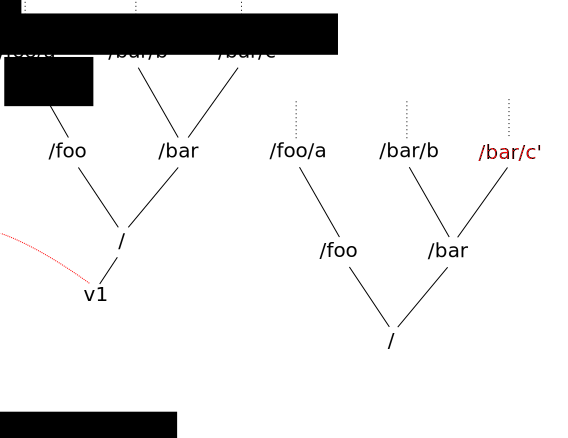
\includegraphics[width=0.85\textwidth]{images/git2.pdf}}%
      \only<+>{\includegraphics[width=0.85\textwidth]{images/git3.pdf}}%
      \only<+>{\includegraphics[width=0.85\textwidth]{images/git4.pdf}}%
      \only<+>{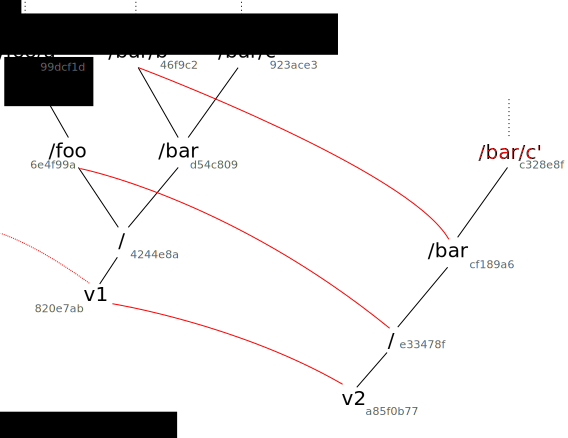
\includegraphics[width=0.85\textwidth]{images/git5.pdf}}%
      \only<+>{\includegraphics[width=0.85\textwidth]{images/git6.pdf}}%
      \only<+>{\includegraphics[width=0.85\textwidth]{images/git7.pdf}}%
    \end{center}
  \end{onlyenv}
  \begin{onlyenv}<8->
    The repository $R$ is a pair $(\Delta, x)$:
    \[ \Delta : x \mapsto (\mathsf{Commit}\ (x\times y) \gor \mathsf{Tree}\ \vec x
    \gor \mathsf{Blob}\ string)\]
    \begin{overlayarea}{\textwidth}{12em}
      \begin{onlyenv}<8>
        \begin{block}{Operations}
          \begin{description}
          \item[\texttt{commit $\delta$}]
            \begin{itemize}
            \item extend the database with \textsf{Tree}/\textsf{Blob}
              objects
            \item add a \textsf{Commit} object
            \item update head
            \end{itemize}
          \item[\texttt{checkout $v$}]
            \begin{itemize}
            \item follow $v$ all the way to the \textsf{Blob}s
            \end{itemize}
          \item[\texttt{diff $v_1$ $v_2$}]
            \begin{itemize}
            \item follow simultaneously $v_1$ and $v_2$
            \item if object names are equal, stop (content is equal)
            \item otherwise continue
            \end{itemize}
          \item[\dots]
          \end{description}
        \end{block}
      \end{onlyenv}
      \begin{onlyenv}<9->
        \begin{block}{Invariants}
          \begin{itemize}
          \item $\Delta$ forms a DAG
          \item if $(x, \mathsf{Commit}\ (y,z)) \in\Delta$ then
            \begin{itemize}
            \item $(y, \mathsf{Tree}\ t)\in\Delta$
            \item $(z, \mathsf{Commit}\ (t,v))\in\Delta$
            \end{itemize}
          \item if $(x, \mathsf{Tree}(\vec y))\in\Delta$ then \\
            for all $y_i$, either $(y_i, \mathsf{Tree}(\vec z))$ or
            $(y_i, \mathsf{Blob}(s))\in\Delta$
          \end{itemize}
        \end{block}
    \begin{onlyenv}<10>
      \begin{center}
        {\Large Let's do the same with \emph{proofs}}
      \end{center}
    \end{onlyenv}
      \end{onlyenv}
    \end{overlayarea}
  \end{onlyenv}
\end{frame}

\begin{frame}[fragile]{A \emph{typed} repository of proofs}
  \begin{center}
    \only<+>{\includegraphics[width=0.85\textwidth]{images/gasp1.pdf}}%
    \only<+>{\includegraphics[width=0.85\textwidth]{images/gasp2.pdf}}%
    \only<+>{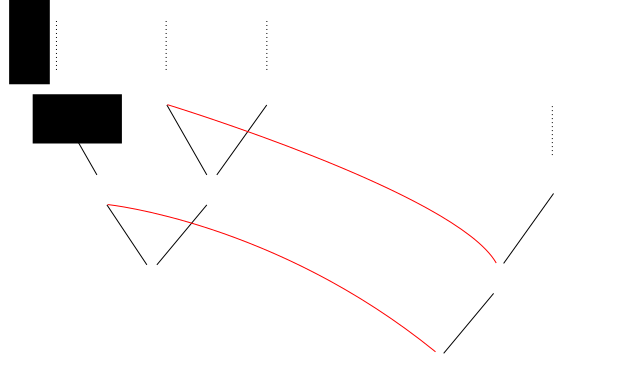
\includegraphics[width=0.85\textwidth]{images/gasp3.pdf}}%
    \only<+>{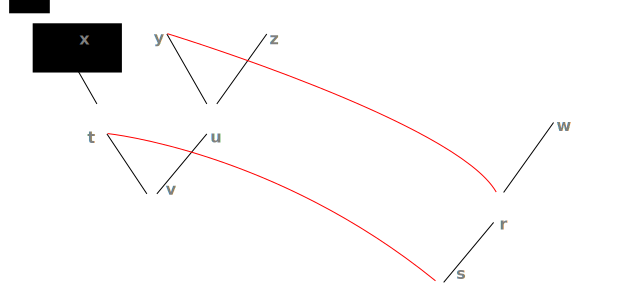
\includegraphics[width=0.85\textwidth]{images/gasp4.pdf}}%
    \only<+>{\includegraphics[width=0.85\textwidth]{images/gasp5.pdf}}%
  \end{center}
\end{frame}

\begin{frame}{A data-oriented notion of delta}
  \begin{block}{The \alt<+>{first-order}{binder} case}
    \begin{overlayarea}{\textwidth}{10em}
      \alt<1>
      {\vspace{0.6em}\centering\includegraphics[width=0.90\textwidth]{images/delta.png}\\}%
      {\hspace{1em}\centering\includegraphics[width=0.90\textwidth]{images/delta2.png}\\}%
    \end{overlayarea}
    A delta is a term $t$ with \emph{metavariables} \alert{$\mmeta,
      \mmmeta$}
    \alt<1>{, defined in the repository}{and \emph{boxes} \alert{$\ibox t \mmeta y u$} to
      jump over binders in the repository}
  \pause
  \end{block}
\end{frame}

\begin{frame}{Towards a metalanguage of proof repository}
  \begin{block}{Repository language}
    \begin{enumerate}
    \item name all proof steps
    \item annote them by judgement
    \end{enumerate}
  \end{block}
  \begin{block}{Delta language}
    \begin{enumerate}
    \item address sub-proofs (metavariables)
    \item instantiate lambdas (boxes)
    \item check against $\mr$
    \end{enumerate}
  \end{block}
  \pause
  $\leadsto$ \bf Need extra-logical features!
\end{frame}

\subsection{Logical framework}

\begin{frame}{\gray{A} logical framework \gray{for incremental type-checking}}
  \begin{onlyenv}<-2>
    LF \cit{Harper et al. 1992} (a.k.a. $\lambda\Pi$) provides a {\bf
      meta-logic} to represent and validate syntax, rules and proofs
    of an \textbf{object language}, by means of a typed
    $\lambda$-calculus.

    \begin{description}
    \item[Dependent types] to express object-judgements
    \item[Signature] to encode the object language
    \item[HOAS] to easily manipulate hypothesis
    \end{description}
    \pause
    \begin{example}
      \scriptsize
      \[
      \begin{array}{c}
        [x:A]\\
        \vdots\\
        t : B \\\hline
        \ulam x t : A\to B
      \end{array}
      \qquad\leadsto\qquad
      \begin{array}{l}
        \prd {A,B}{ty} \prd t {tm\to tm} \\
        (\prd x {tm} {\textsf{is}\ x\ A} \to \textsf{is}\ (t\ x)\ B) \to \\
        \textsf{is}\ (\textsf{lam}\ A\ (\ulam x t\ x))(\textsf{arrow}\ A\ B)
      \end{array}
      \]
    \end{example}
  \end{onlyenv}
  \begin{onlyenv}<3>
    \begin{block}{\textsf{Twelf}'s use}
      \begin{enumerate}
      \item encode language \& typing rules (signature)
      \item prove inductive properties (signature)
      \item verify well-typing, termination \& coverage
      \end{enumerate}
    \end{block}
    \begin{block}{Our use}
      \begin{enumerate}
      \item encode language \& typing rules (signature)
      \item write object language derivation deltas (term)
      \item check deltas \emph{wrt.} signature
      \item GOTO 2
      \end{enumerate}
    \end{block}
  \end{onlyenv}
  \begin{onlyenv}<4>
    \inXLF
    \begin{block}{Syntax}
      \begin{align*}
        \mk &\gequal { \prd\mv\mf\mk \gor \type } \\
        \mf &\gequal { \prd\mv\mf\mf \gor \app\mf\mo \gor \mcf } \\
        \mo &\gequal { \lam\mv\mf\mo \gor \app\mo\mo \gor \mv \gor \mco } \\[0.5em]
        \msi &\gequal { \enil \gor \ebinddecl\msi\mco\mf \gor
          \ebinddecl\msi\mcf\mk }
      \end{align*}
    \end{block}
    \begin{block}{Judgements}
      \begin{itemize}
      \item $\jindex\msi\me K$
      \item $\jindex\msi\me {\typ A K}$
      \item $\jindex\msi\me {\typ t A}$
      \item $\vdash \msi$
      \end{itemize}
    \end{block}
  \end{onlyenv}
\end{frame}

\begin{frame}{The delta language}
  \inXLF
  \begin{columns}
    \begin{column}{0.6\textwidth}
      \begin{block}{Syntax} \vspace{-2em}
        \begin{align*}
          \mk &\gequal { \prd\mv\mf\mk \gor \type } \\
          \mf &\gequal { \prd\mv\mf\mf \gor \app\mf\mo \gor \mcf } \\
          \mo &\gequal { \lam\mv\mf\mo \gor \app\mo\mo \gor \mv \gor \mco
            \gor \alert{\mmeta \gor \ibox\mo\mmeta\mv\mo}
          } \\[0.5em]
          \msi &\gequal { \enil \gor \ebinddecl\msi\mco\mf \gor
            \ebinddecl\msi\mcf\mk }
        \end{align*}
      \end{block}
    \end{column}
    \begin{column}{0.4\textwidth}
      \begin{block}{Judgements}
        \begin{itemize}
        \item $\jindex\msi{\pair{\alert\mr}\me}\mk\alert{\To\mr}$
        \item $\jindex\msi{\pair{\alert\mr}\me}{\typ\mf\mk}\alert{\To\mr}$
        \item $\jindex\msi{\pair{\alert\mr}\me}{\typ\mo\mf}\alert{\To\mr}$
        \item $\vdash\msi\alert{\To\mr}$
        \end{itemize}
      \end{block}
    \end{column}
  \end{columns}
  \begin{block}{Informally}
    \begin{itemize}
    \item $\jindex\msi{\pair\mr\me}\mmeta\To\mmr$ {\footnotesize
        means}\\ “I am what $\mmeta$ stands for in $\mr$ (and produce $\mmr$)”.
    \item $\jindex\msi{\pair\mr\me}{\ibox\mo\mmeta\mv\mmo}\To\mmr$ {\footnotesize
        means}\\ “Meta $\mmeta$ has the form $\ulam \mv\ldots$ in $\mr$. Make all
      metavariables under this lambda in scope for $\mo$, taking
      $\mmo$ for $\mv$. $\mo$ will produce $\mmr$”
    \end{itemize}
  \end{block}
\end{frame}

\begin{frame}{The repository language}
  
\end{frame}

\begin{frame}{Commit/Checkout}
  
\end{frame}

\begin{frame}{Example}
  
\end{frame}

\begin{frame}{Regaining version management}
  
\end{frame}

\begin{frame}{A word on \textsf{ti}}
  
\end{frame}

\begin{frame}{Further work}
  
\end{frame}

%  But
%   we need a little bit more: \\[1em]

%   {\small\textsf{
%       \noindent\ldots\\
%       \alert<2>{\textbf{let}} \alert<5>u = \alert<4>{pair y z} : \alert<3>{is nil (conj A B)} \textbf{in}\\
%       \hspace{2ex}\textbf{let} \alert<5>v = app t u : is nil C \textbf{in}\\
%       \ldots
%   }}
% \pause
% \begin{enumerate}[<+->]
% \item definitions / explicit substitutions
% \item type annotations on application spines
% \item fully applied constants / $\eta$-long NF
% \item Naming of all application spines / A-normal form\\
%   {\footnotesize(= construction of syntax/proofs)}
% \end{enumerate}

% \subsection{Positionality}

% \begin{frame}[fragile]{Positionality}
% $R =$ \scriptsize
% \begin{lstlisting}
%     let x = ... : is (cons (conj A B) nil) C in
%       let y = ... : is nil A in
%         let z = ... : is nil B in
%           let t = lam (conj A B) x : is nil (arr (conj A B) C) in
%             let u = pair y z : is nil (conj A B) in
%               let v = app t u : is nil C in
%                 let w = commit v w1 : version in
%                   w
% \end{lstlisting}
% \normalsize
% \pause
% \begin{itemize}
% \item Expose the \emph{head} of the term
% \pause {\Large \[(\lambda x.\lambda y. T)\ U\ V\]}
% \item \pause Abstract from the \emph{positions} of the binders \\
%   {\footnotesize (from inside and from outside)}
% \end{itemize}
% \end{frame}








%   \begin{onlyenv}<6-9>
%     \small
%     \begin{overlayarea}{0pt}{\textheight}
%       \begin{align*}
%         x &= \ldots\ : A\wedge B\vdash C \\
%         y &= \ldots\ :\ \vdash A \\
%         z &= \ldots\ :\ \vdash B \\
%         t &= \lam a {A\wedge B} x :\ \vdash A\wedge B\to C \\
%         u &= (y, z) :\ \vdash A\wedge B \\
%         v &= \app t u :\ \vdash C \\
%         w &= \mathsf{Commit}(v,w1) : \mathsf{Version} \only<7>{
%           \alert{\qquad,\quad w} }
%         \only<8-9>{ \\
%           p &=\ldots\ :\ \vdash B \\
%           q &= (y, p) :\ \vdash A \wedge B \\
%           r &= \app t q :\ \vdash C \\
%           s &= \mathsf{Commit}(r,w) : \mathsf{Version} \only<9>{
%             \alert{\qquad,\quad s} } }
%       \end{align*}
%     \end{overlayarea}
%   \end{onlyenv}
%   \begin{onlyenv}<10->
% \footnotesize
% \begin{uncoverenv}<12>
% \begin{lstlisting}
% ...
% val is : env -> prop -> type
% val conj : prop -> prop -> prop
% val pair : is 'a 'b -> is 'a 'c -> is 'a (conj 'b 'c)
% val version : type
% val commit : is nil C -> version -> version
% ...
% \end{lstlisting}
% \end{uncoverenv}
% \begin{overlayarea}{\textwidth}{\textheight}
% \begin{onlyenv}<10>
% \begin{lstlisting}
% let x = ... : is (cons (conj A B) nil) C in
%   let y = ... : is nil A in
%     let z = ... : is nil B in
%       let t = lam (conj A B) x : is nil (arr (conj A B) C) in
%         let u = pair y z : is nil (conj A B) in
%           let v = app t u : is nil C in
%             let w = commit v w1 : version in
%               w
% \end{lstlisting}
% \end{onlyenv}
% \begin{onlyenv}<11->
% \begin{lstlisting}
% let x = ... : is (cons (conj A B) nil) C in
%   let y = ... : is nil A in
%     let z = ... : is nil B in
%       let t = lam (conj A B) x : is nil (arr (conj A B) C) in
%         let u = pair y z : is nil (conj A B) in
%           let v = app t u : is nil C in
%             let w = commit v w1 : version in
%               let p = ... : is nil B
%                 let q = pair y p : is nil (conj A B) in
%                   let r = t q : is nil C
%                     let s = commit r w : version in
%                       s
% \end{lstlisting}
% \end{onlyenv}
% \end{overlayarea}
%   \end{onlyenv}

\end{document}

%%% Local Variables: 
%%% mode: latex
%%% TeX-master: t
%%% End: 
